\newpage
\thispagestyle{sectioned}
\chapter{Construyendo la idea de la aplicación: DemoCritics}

\section{Introducción}

Una vez que habíamos migrado la tecnología de Wave que soportaría el núcleo de nuestra aplicación, era hora de decidir qué aplicación le íbamos a dar de cara a desarrollar una aplicación Android que hiciera uso de ello. Era importante tener en cuenta las características que nos ofrecía Wave:

 - Edición colaborativa.

 - Consistencia en Tiempo Real.
 
\subsubsection{Brainstorming de ideas}

Un \textit{brainstorming} \cite{ref:bookBrainStorming} (o lluvia de ideas en español) es una técnica de trabajo en grupo que persigue que todos sus integrantes se junten para generar ideas originales en un ambiente distendido. El objetivo es primar la cantidad por encima de la calidad de éstas para después de la sesión realizar un proceso de selección de las más interesantes. De esta manera pueden salir ideas que a priori podrian resultar absurdas pero que otros integrantes del grupo pueden aprovechar para que surjan otras nuevas.  

Después de considerar posibles ideas de implementaciones que podrían hacer uso de estas características, decidimos realizar una sesión de \textit{brainstorming} junto a nuestros directores de proyecto para identificar ideas potenciales. En esta sesión aparecieron temas tan variados como wikis colaborativas, aplicaciones de inteligencia artificial, aportaciones colaborativas en política, edición de vídeos y música, cursos de formación colaborativos, visualizacion de mapas, etc.

	\begin{figure}[H]
        \centering
        \begin{subfigure}[b]{0.7\textwidth}
                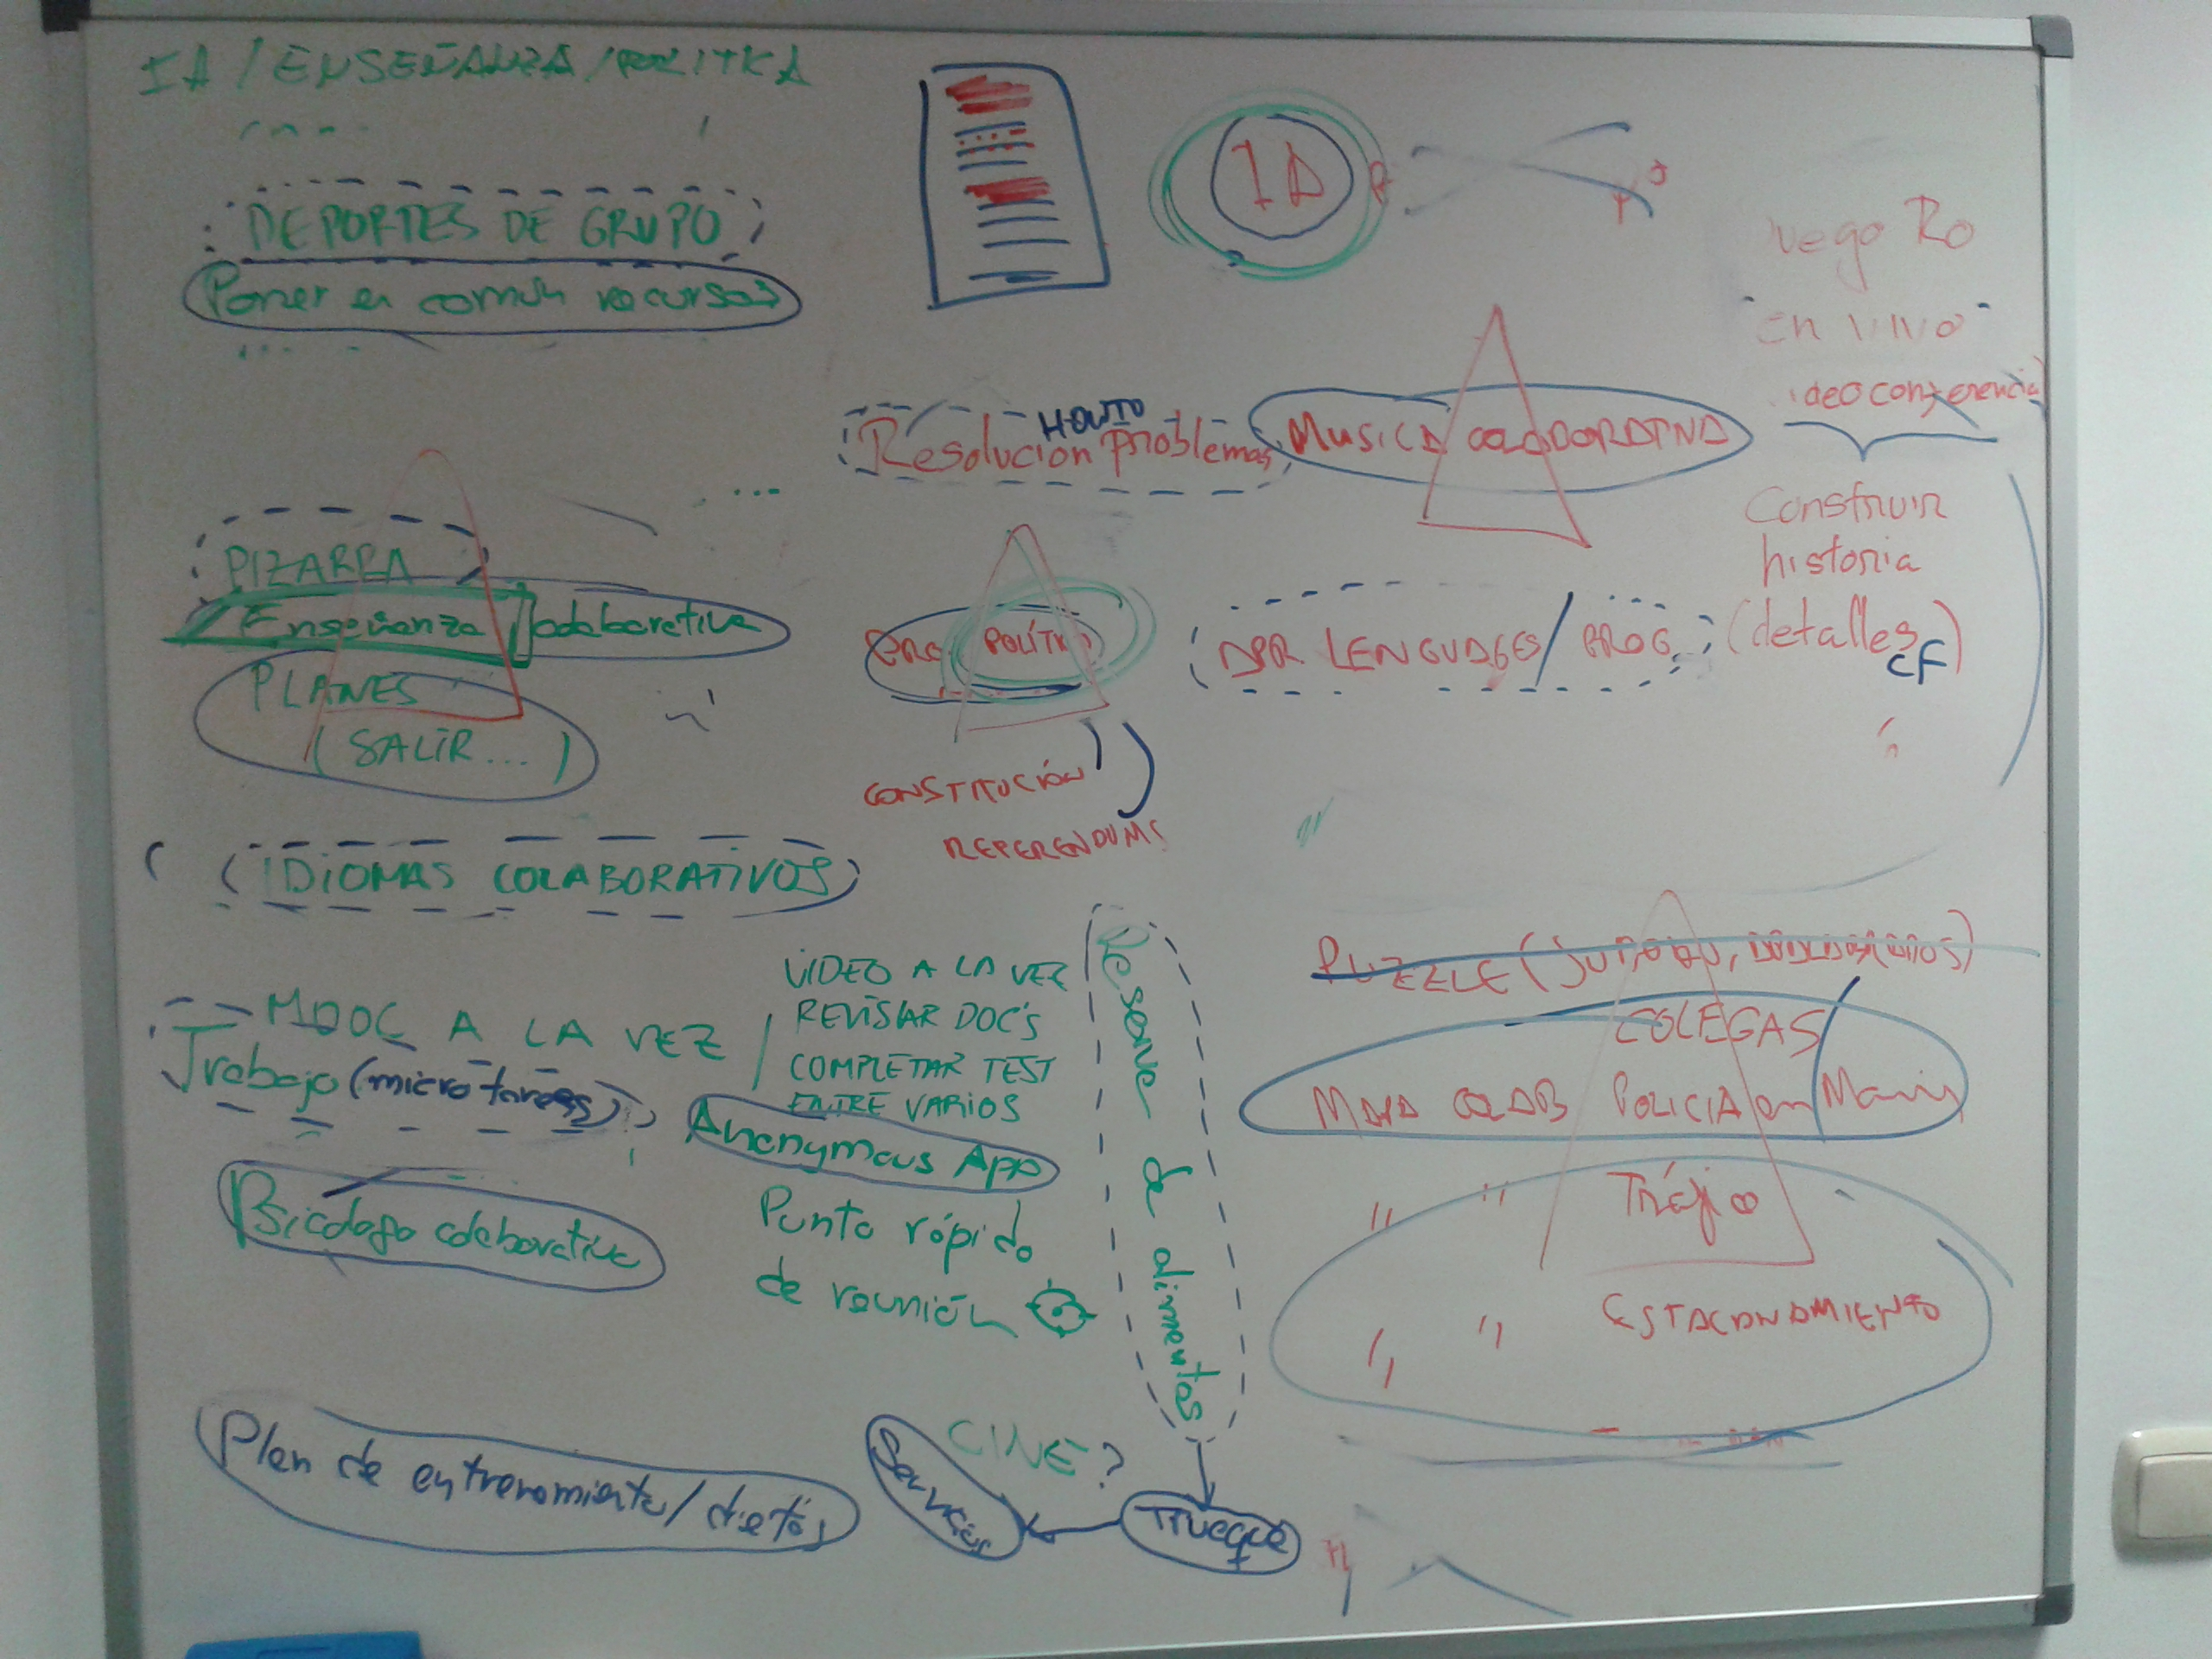
\includegraphics[width=\textwidth]{Media/Captures/brainstorming.jpg}
                \caption{Idea de Aplicación}
                \label{fig:brainstormingApp}
        \end{subfigure}
        ~
        \begin{subfigure}[b]{0.7\textwidth}
                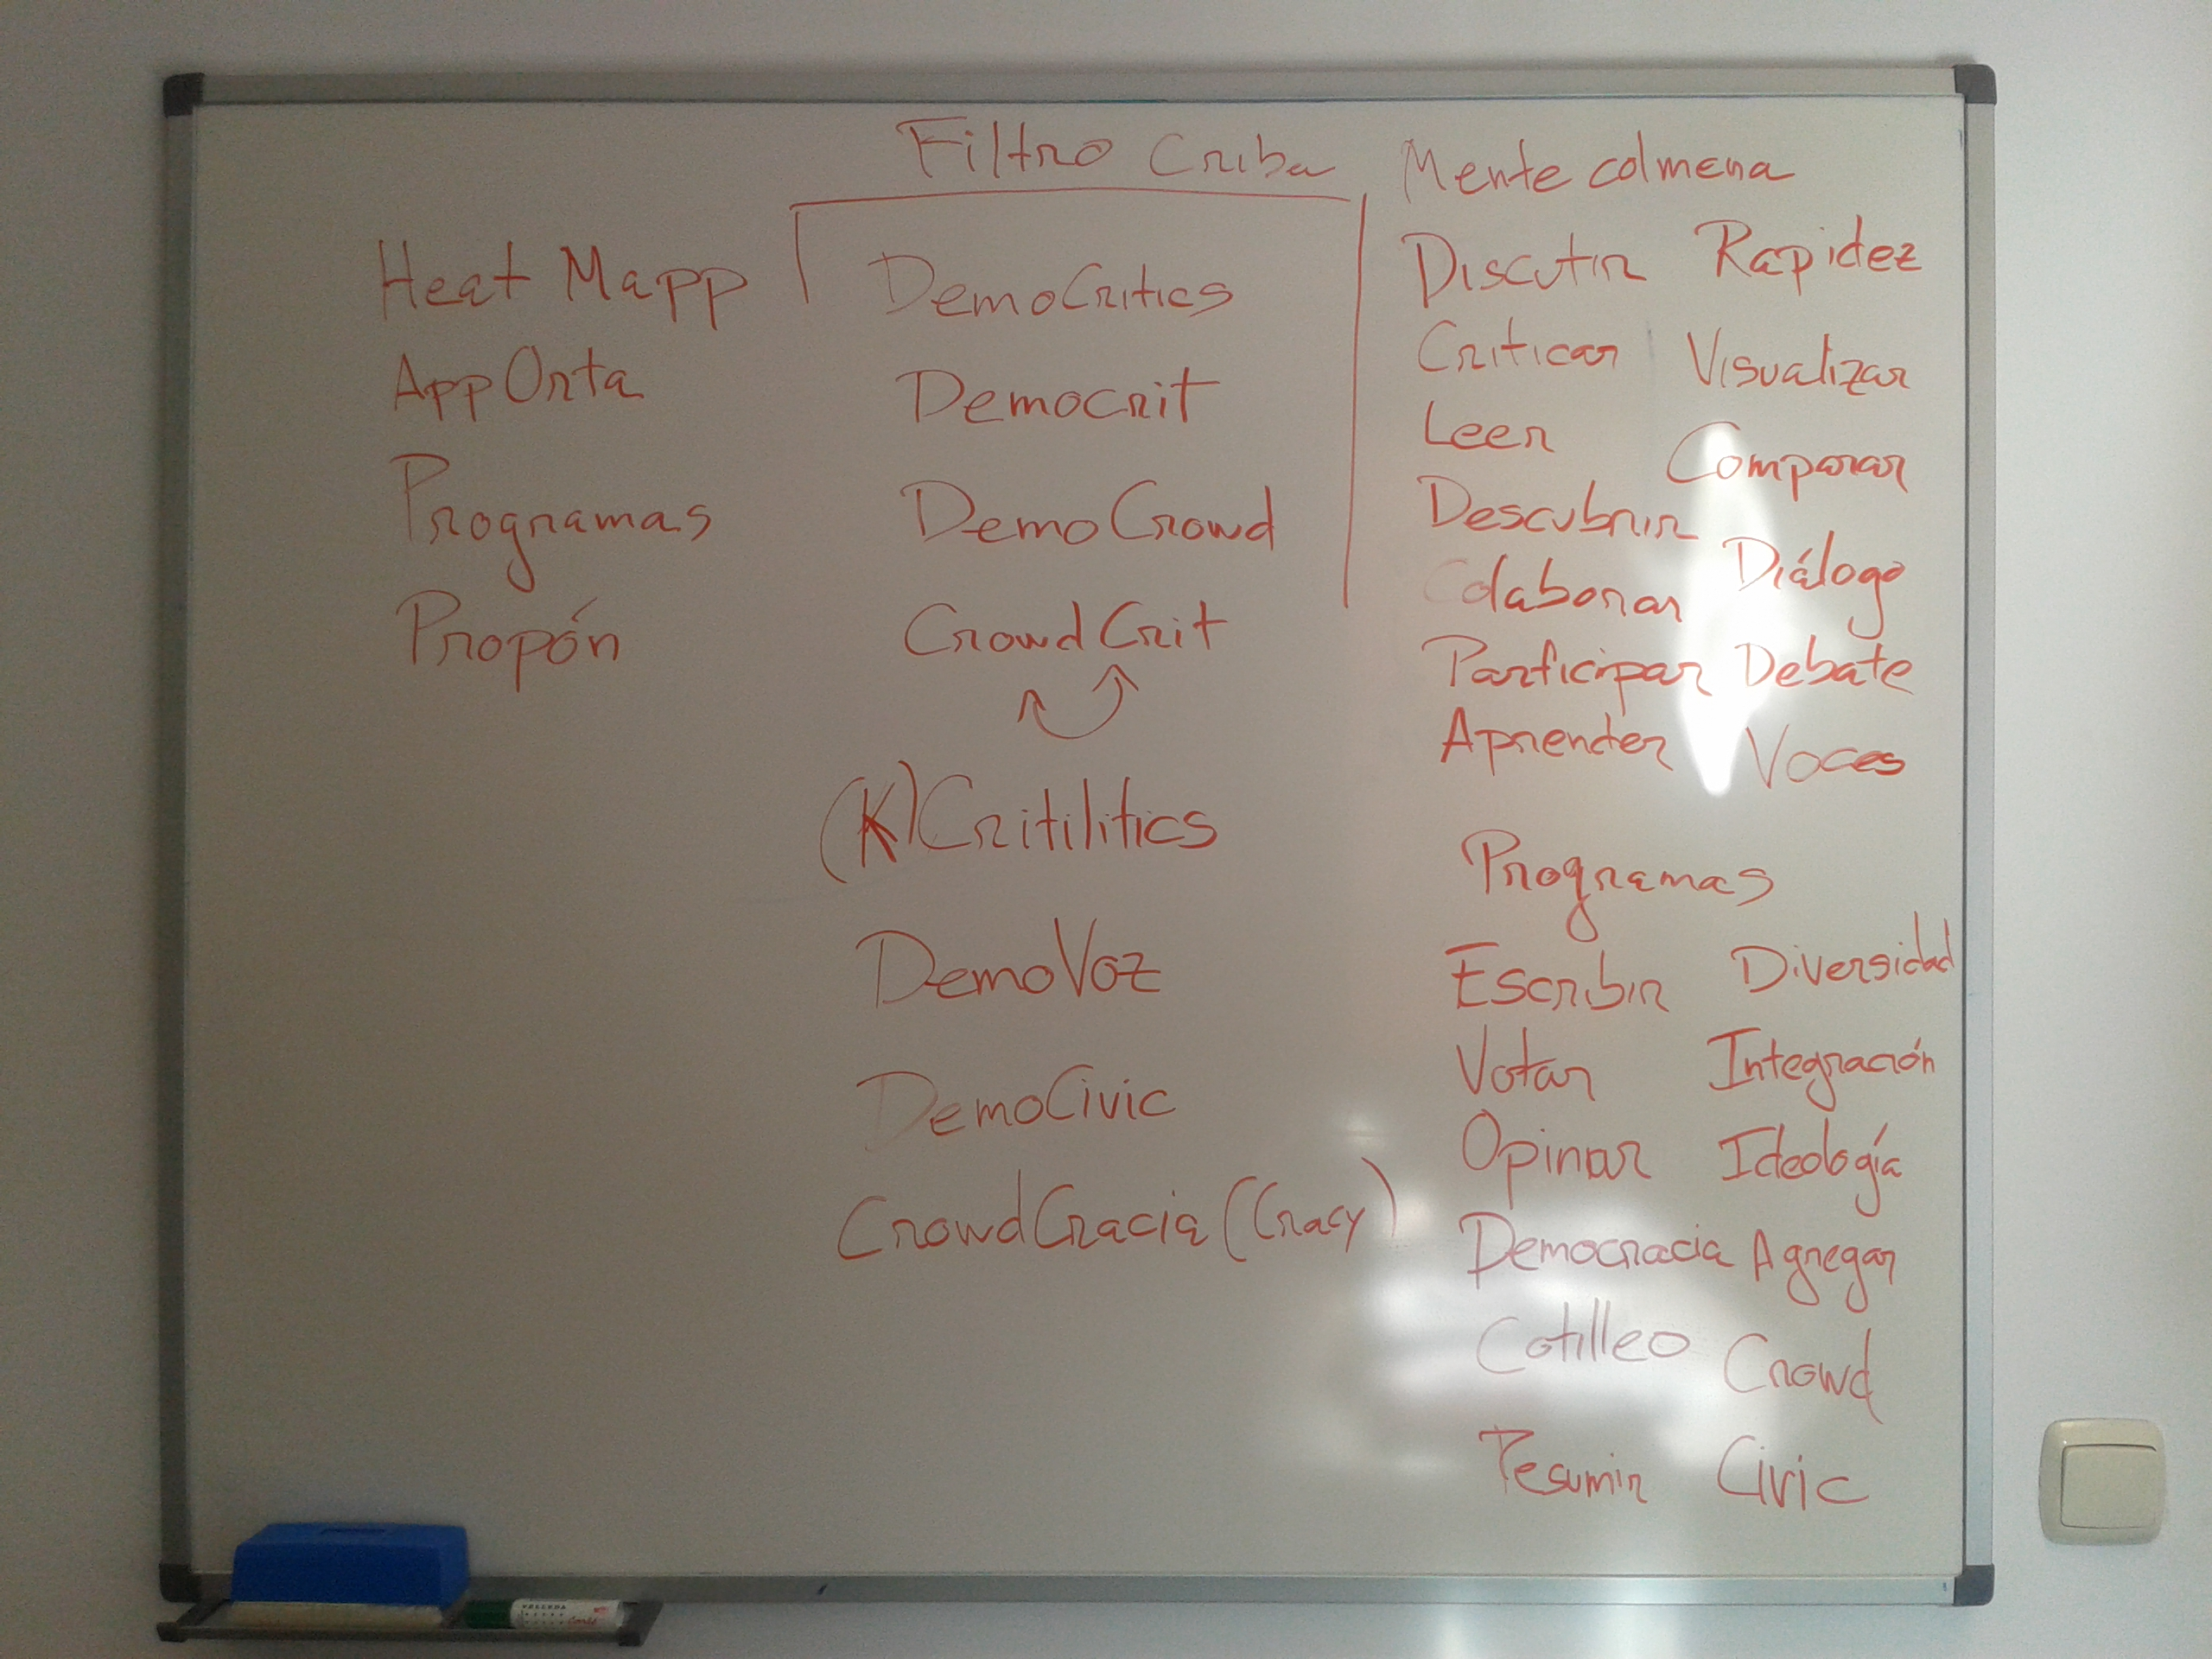
\includegraphics[width=\textwidth]{Media/Captures/appname.jpg}
                \caption{Posibles Nombres}
                \label{fig:brainstormingName}
        \end{subfigure}
        \caption{Capturas del brainstorming}\label{fig:brainstormingCaptures}
	\end{figure}
	


Con un gran repertorio de ideas expuestas en la sesión, decidimos centrarnos primero en descartar aquellas que a nosotros no nos motivaba llevar a cabo. De esta manera nos quedamos con cuatro ideas fundamentales a desarrollar en nuestra aplicación: Política, Música, Inteligencia Artificial y Mapas. Centrándonos ahora solo en estos temas, surgieron varias ideas colaborativas como: desarrollar documentos políticos, programas electorales, comunicación entre colectivos en tiempo real, aprendizaje de música, edición de partituras y obras, aplicaciones colaborativas con inteligencia artificial, edición de mapas en tiempo real, lexicalización, etc.

Finalmente, ya que ambos teníamos interes por la política, decidimos realizar una aplicación colaborativa relacionada con dicho mundo. En esta aplicación podríamos recurrir a la edición de contenidos en tiempo real, ya fueran propuestas políticas, programas electorales u otro tipo de documentos. Más adelante también podríamos hacer uso incluso de alguna herramienta de Inteligencia Artificial para automatizar algunas tareas o realizar recomendaciones sociales.

Lo que sí que tuvimos claro desde el principio es la idoneidad del momento actual para desarrollar una aplicación de temática política, dado que nos encontramos en año electoral. Nos propusimos el objetivo de desarrollar algo que pudiera tener cierta repercusión y utilidad en las próximas citas electorales de este año 2015. Intentariamos pensar en la aplicación no solo como un Trabajo de Fin de Grado sino como algo que pudiéramos llevar más allá y que resultara útil a la sociedad.

Por otro lado, queriamos elegir un nombre para la aplicación que fuera a la vez atractivo y significativo de la participación ciudadana que representa. Para esto hicimos tambien una sesión de \textit{brainstorming} con varias personas, de la cual sacamos varias posibilidades por el nombre. Tras someter a votación estos nombres nos quedamos con el que más gustó a todos: \textbf{DemoCritics}.

\section{Marco teórico de la idea}

En los siguientes puntos se discutirá acerca de una serie de consideraciones sobre el estado actual de la política y la democracia. Nos centraremos sobre todo en su relación con las nuevas tecnologías como herramientas capaces de cambiar la manera en la que se conciben ambas disciplinas.

\subsection{Política en el mundo de la Informática}

A primera vista podemos pensar que la informática no parece entusiasmar a los informáticos. Podemos ubicar la política como una parte de las ciencias sociales, situando la informática en ciencias formales. Pero si pensamos en factores como la gestión de los privilegios de una aplicación entre los que definiremos de alguna forma una jerarquía, estaremos en cierta manera haciendo política. También encontraremos características políticas en el diseño relacional de una base de datos. Definiendo los campos de una base de datos podemos encontrarnos con algunos valores como el sexo, la nacionalidad, la edad o incluso las relaciones o restricciones que existen entre las tablas. Estaremos definiendo unas reglas básicas de funcionamiento de la base de datos establecidas por unos principios políticos.

Además si nos sumergimos en el mundo de las Licencias de Uso en el desarrollo de \textit{Software} encontraremos más política aún. Licencias que determinan el uso de un tipo de \textit{Software}, ya sea para compartir, vender o distribuir copias. Multitud de reglas políticas definidas en un documento de licencia de uso. Así como las restricciones que establecemos en la metodología orientada a objetos, estableciendo las relaciones de herencia, restricción de métodos, variables, etcétera.

Regresando a la actualidad y basándonos en no muy lejanos acontecimientos pasados, habremos oído cómo algunos gobiernos recopilan datos de la actividad de los usuarios en las redes sociales \cite{ref:NSAData}, analizando todo el contenido que generan. Incluso vemos cómo algunas aplicaciones móviles piden aprobar permisos con los que operar libremente en tu dispositivo.

Observamos por tanto que la política está más integrada en la informática de lo que parece, sobre todo si dejamos a un lado la informática más científica y formal y pasamos a la informática social, la de los gobiernos, la de los negocios o la de las relaciones sociales.


\section{Adentrándonos en la idea}

La idea a desarrollar está generada en una época en la que la política parece haber despertado el interés de una parte considerable de la ciudadanía. Podría ser por tanto una herramienta útil para participar en temas políticos de forma sencilla y atractiva. Dejando así atrás los tópicos a menudo escuchados de \textit{"yo no entiendo de política"}, \textit{"la política es aburrida"}, \textit{"no sé a quién votar"} o \textit{"no he leído nunca un programa electoral"} entre otros.

La herramienta ofrecería una nueva forma de participar en la política y de llevar a los ciudadanos los programas electorales expuestos por las diferentes formaciones políticas. De forma que, para potenciar el uso social de la aplicación, los ciudadanos podrían leer aquellos puntos de los programas más vistos, debatidos, comentados, etc. Así, cualquier usuario tendría a su disposición todos los programas electorales en su bolsillo, por lo que no tendría que ir a la página web de cada formación política y descargarse un documento de 200 páginas. Pensamos que esta forma tradicional de presentar un programa político en un solo documento en un mundo donde las posibilidades de comunicarnos se han desarrollado exponencialmente mediante las nuevas tecnologías no es la mejor manera de generar interés por su lectura y la implicación en política de las personas.

Por otra parte, y teniendo en cuenta la tendencia actual de los nuevos movimientos ciudadanos de elaborar programas políticos en base a propuestas de los ciudadanos, \textbf{la aplicación también debía ofrecer alguna manera de realizar Propuestas y debatirlas entre todos}. De esta forma tanto la ciudadanía como las formaciones políticas podrían saber en cualquier momento cuáles son las principales preocupaciones de los ciudadanos y qué medidas o soluciones proponen para resolverlas. \textbf{Además pensamos que podríamos aprovechar las características de Wave para realizar estas Propuestas de forma colaborativa y en tiempo real}, aportando un valor diferenciador respecto a las actuales soluciones desarrolladas para web (Ver sección \ref{ssec:artProposals}).

Por tanto, desde un primer punto de vista subjetivo, la aplicación quedó dividida en dos partes. Por un lado tendríamos la presentación estructurada de los programas políticos que presentan las formaciones políticas. Y por otro todas las propuestas que elaboran de forma colaborativa los ciudadanos, ya sea individualmente o en colectivos sociales.



